\documentclass[USenglish]{ifimaster}  %% ... or USenglish or norsk or nynorsk
\usepackage[utf8]{inputenc}           %% ... or latin1
\usepackage[T1]{fontenc,url}
\usepackage{todonotes}
\urlstyle{sf}
\usepackage{babel,textcomp,csquotes,duomasterforside,varioref,graphicx}
\usepackage[backend=biber,style=numeric-comp]{biblatex}
\usepackage{acronym}
%\setcounter{tocdepth}{5}

\title{Image-based terrain characterization for autonomous vehicles, based on deep learning}        %% ... or whatever

\author{Andreas Hagen}                      %% ... or whoever 

\bibliography{references.bib}                  %% ... or whatever

\begin{document}
\duoforside[dept={Department of Technology Systems},   %% ... or your department
  program={Cybernetics},  %% ... or your programme
  short]                                        %% ... or long

\frontmatter{}
\chapter*{Abstract}                   %% ... or Sammendrag or Samandrag

\tableofcontents{}
\listoffigures{}
\listoftables{}

\chapter*{Preface}
%\addcontentsline{toc}{chapter}{Abbreviations} \noindent
%--- Acronyms -----------------------------------------------------------------%
% \acrodef{label}[acronym]{written out form} % acronym syntax
%\acrodef{etacar}[$\eta$ Car]{Eta Carinae}   % acronym example
%--- Acronyms -----------------------------------------------------------------%
% how to use acronyms:
% \ac = use acronym, first time write both, full name and acronym
% \acf = use full name (text + acronym)
% \acs = only use acronym
% \acl = only use long text
% \acp, acfp, acsp, aclp = use plural form for acronym (append 's')
% \acsu, aclu = write + mark as used
% \acfi = write full name in italics and acronym in normal style
% \acused = mark acronym as used
% \acfip = full, emphasized, plural, used
%--- Acronyms -----------------------------------------------------------------%
\chapter*{Abbreviations}
\begin{acronym}
        \acro{ai}[AI]{Artificial intelligence}
        \acro{ann}[ANN]{Artificial Neural Network}
        \acro{dl}[DL]{Deep learning}
        \acro{ml}[ML]{Machine learning}
        \acro{cpu}[CPU]{Central Processing Unit}
        \acro{gpu}[GPU]{Graphics Processing Unit}
        \acro{rgb}[RGB]{Red,Green,Blue}
\end{acronym}


\mainmatter{}
\chapter{Introduction}                  
\section{Motivation}
\section{Background}
\section{Problem description}
\section{Thesis outline}

\chapter{Theoretical background}
% Write about 3 things: General info on deep learning and computer vision, other persons work, mathematical background
This chapter will provide an overview of the basics of \ac{ai}, \ac{ml}, and \ac{dl}. These fields and techniques are the basis for this thesis. Then cover the necessary remaining theory and mathematics related to the thesis, and lastly go over related works. \todo{gjør om etter kapittelet er ferdigskrevet}
\section{Artificial intelligence}
\ac{ai} is a field where machines are able to demonstrate intelligence through mathematics, statistics and logic. It has the ability to tackle many complex problems that are intellectually difficult or impossible to solve for a human being with natural intelligence. Even though \ac{ai} could solve complex problems, it still had a few challenges in the early days. Some intuitive tasks for us, like recognizing a cat or a dog in an image or the context of a written text, proved to be a true challenge. A solution to these problems was to allow machines to learn from experience, which is where \ac{ml} and \ac{dl} comes into the picture\cite{The_holy_grail_of_DL}.
\begin{figure}[ht]
    \centering
    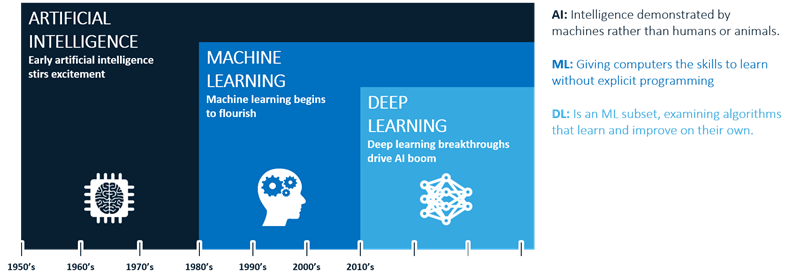
\includegraphics[width=0.8\textwidth]{bilder/AI_ML_DL.png}
    \caption{The history of AI, ML, and DL
    \protect\cite{website:AI}}
    \label{fig:AI}
\end{figure}
\subsection{Machine learning}
Figure \ref{fig:AI} illustrates that \ac{ml} is a subset from \ac{ai}. Instead of solve the task with explicit instructions, \ac{ml} learns from experience.
\todo{mere juice}
\subsection{Deep learning}
Instead of learning from specific tasks like in \ac{ml}, \ac{dl} learns data representations from data sets. Both \ac{ml} and \ac{dl} learns from unsupervised-, semi-supervised- or supervised learning. \todo{mere juice}
\subsubsection{Supervised learning}
Supervised learning is the most commonly used technique in \ac{dl} \cite{Francois_Deep_learning_with_python}. The word supervised refers to known targets or annotations in the form of a labelled data set. With that knowledge a function can learn how to map input data to the targets. \todo{sett inn formel og forklar}
\subsubsection{Keras}
Keras is a user-friendly \ac{dl} library developed in Python. It was originally made for researchers as way to do quick experimentation, with an easy implementation. Keras has quickly gained popularity among its users and is one of the most popular framework in \ac{dl} projects nowadays. The main reasons for the popularity is the user-friendliness and that Keras can run with the same code seamlessly on \ac{cpu} or \ac{gpu}\cite{Francois_Deep_learning_with_python}.
\subsection{Benefits using deep learning vs traditional methods}
\section{Computer vision}
Computer vision is a field which main purpose is to make machines be able to interpret and understand features from images or video. Or easier said, "Teaching computers
how to see"\cite{website:maskinsyn-intro}.  
\section{Data preprocessing}
This section will cover data processing from an image-based point of view. Before the data set can be fed into the network, would it in the most cases be inevitable to perform several preprocesses. This is necessary in order to make it ready for training. 
\newline
A common thing to do with an image-based data set is to resize the images to a slightly lower resolution. This is especially necessary if the computer does not have a state-of-art \ac{gpu}, as the model otherwise might be very slow. The down scaling will help the model to be more effective and less time consuming, at the prize of loosing some features from the original resolution. It is therefore important to test different scales, to find the perfect fit between keeping enough key features and have an effective model.
\newline
A \ac{rgb} image contains integer values in the range from 0-255 in each of its three channels. Because the values of the weights in an \ac{ann} is relatively small, it is normal practice to normalize the image-array to values between 0-1. This can be done by divide the array with 255. Doing so will prevent to slow down the learning process, as the values from the weights and the array now are in closer range. Casting the array from int to float before normalizing would increase the accuracy even further. This is due to the float division results in a more accurate number than int division.\todo{legg til bilde eller ligning med forklaring} 
\newline
\newline
Another process is to check whether the data set has the correct shape or not. This is necessary because the network needs to know which input shape to expect. The input layer in Keras is a tensor which are passed to the first hidden layer. If that input layer does not correspond with the shape of each element in the data set, the network will not be able to execute. In the case where "Conv2D" layers are used in a Keras framework, an input array needs to have the following structure:
\newline
\newline
(height, width, channels)
\newline
\newline
Where height and width refers to the x and y coordinates in the image, and channels refers to if the image is binary (channels=1) or \ac{rgb} (channels=3).
\subsection{Data augmentation}
Data augmentation is a helpful tool in order to maintain a more generalized model. It is a method for applying transformations to the training data. When the images are pre-proccessed with the methods described in this section, the network learns how to cope with slightly different images than the original training set. This is the reason the model have a higher chance of predicting the test images (images that the model never have seen before) with more accuracy. In addition to potentially higher accuracy, the model also has lower chance of overfitting. This sub-section will only cover the most used augmentation techniques.  
\subsubsection{Random cropping}
A popular method in augmentation is random cropping. Which means sampling a random chosen square box from the original image, and then resize to the original size.\todo{sett inn bilde} As seen in figure \todo{referer til bildet} the image focus on different areas from the original image, due to the random chosen box. This operation must be included with the ground truth images. When an operation changes the geometry in the image, the same operation must be done in the ground truth image in order to still be a valid target. 
\subsubsection{Flipping images}
Another method is to flip the images in either vertical or horizontal order. Even when the images are flipped, they are still recognizable for the model. The ground truth must also go through the same operation. \todo{sett inn bilde av flipped}Figure \todo{referer til figur} illustrates images with targets being flipped both vertically and horizontally.  
\subsubsection{Color changes}
The idea behind color changes is to make the the model more robust and generalized for new unseen data. Since the geometry in the images are the same after applying color changes, there is not necessary to anything with the ground truth images.
\section{Training, validation and testing data}
\todo{dobbeltsjekk alt fra cs231n, skriv mer ryddig/forståelig}
In order to have a successful implementation, the data set must be split into different parts. Either splitting the data set in training and test, or training, validation and test. The network should only train on the training set, then check accuracy on the validate set and predict values on the testing set. The validation- and test set should be data that the network never has seen before. There is a rule of thumb to split the data in training, validation and test set 60/20/20.  
\todo{skriv om sklearn biblioteket(i metode kap), og hvorfor det er viktig å splitte datasettet korrekt}
\section{Tensorboard}
A handy way to gain control over the training, in order to tweak parameters and control the models accuracy, is using Tensorboard. Tensorboard is a visual tool developed by TensorFlow providing full overview of the training, while training. It is easy to set up in the terminal.
\begin{figure}[ht]
    \centering
    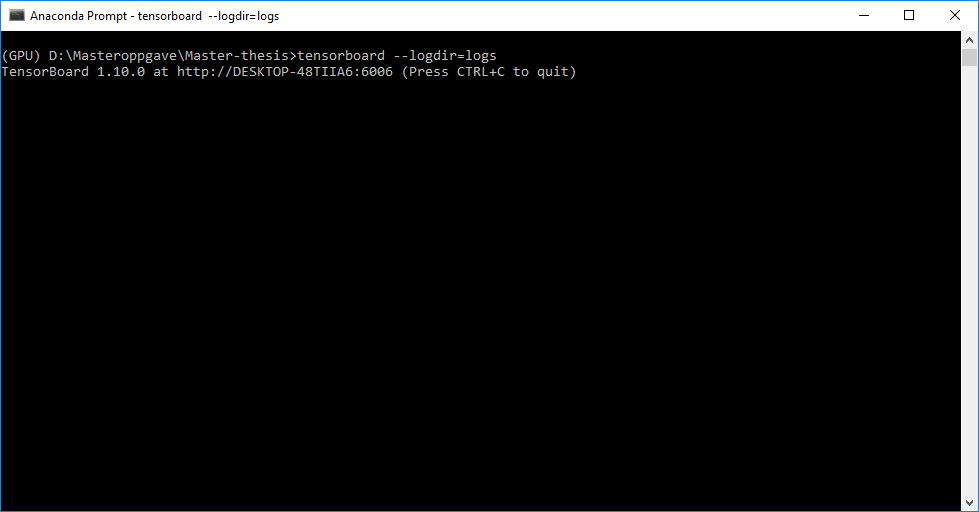
\includegraphics[width=0.8\textwidth]{bilder/tensorboard_anaconda_prompt.PNG}
    \caption{Initializing Tensorboard from terminal}
    \label{fig:tensorboard_anaconda_prompt}
\end{figure}
\newline
As illustrated in figure \ref{fig:tensorboard_anaconda_prompt} Tensorboard is up and running with the command \textit{< tensorboard --logdir=<log> >}. 
\newline
When using Tensorboard with Keras, there is necessary to use callbacks in the code. As stated by the Keras documentation on their website.
\newline
\newline
\textit{"A callback is a set of functions to be applied at given stages of the training procedure. You can use callbacks to get a view on internal states and statistics of the model during training. You can pass a list of callbacks (as the keyword argument callbacks) to the .fit() method of the Sequential or Model classes. The relevant methods of the callbacks will then be called at each stage of the training."}\cite{website:Keras_doc}. 
\newline
\newline
It is therefore possible with callbacks to decide by own specifications what to include and when to gain information during the training process.  
\begin{figure}[ht]
    \centering
    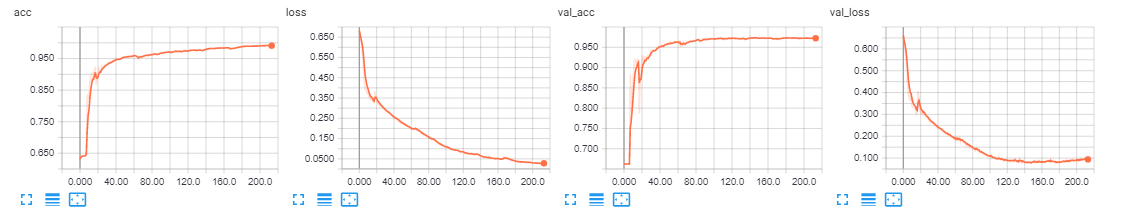
\includegraphics[width=1\textwidth]{bilder/tensorboard_acc_loss.PNG}
    \caption{Accuracy and loss for both training and validation visualized in Tensorboard}
    \label{fig:accuracy_loss}
\end{figure}
\newline
Two popular graphs used to check the quality of the \ac{dl} model is \textit{"accuracy"} and \textit{"loss"}, which are found under the section \textit{"SCALARS"}. 
\begin{figure}[ht]
    \centering
    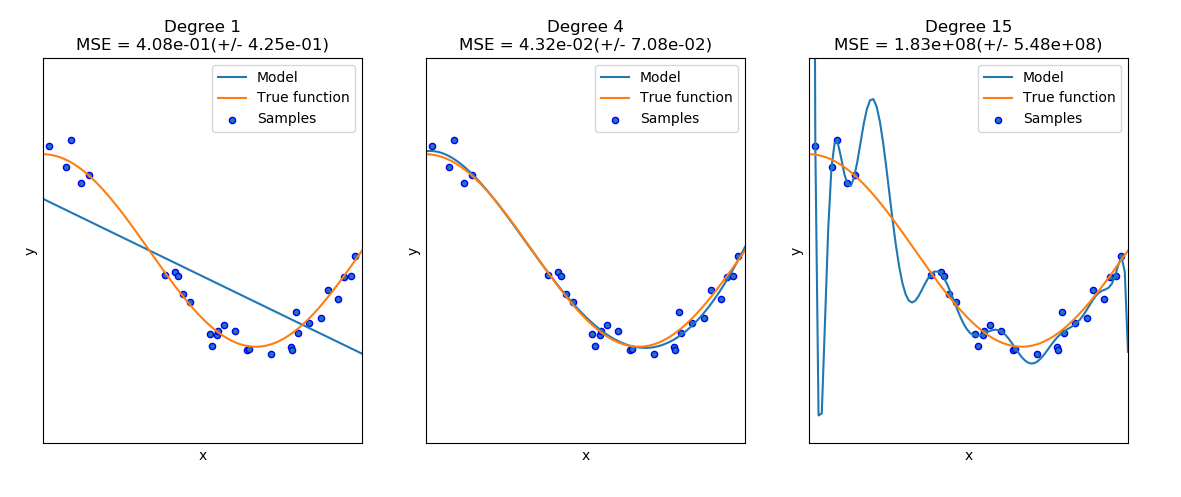
\includegraphics[width=1\textwidth]{bilder/overfitting_underfitting.png}
    \caption{Underfitting, perfect sampling and overfitting \cite{website:overfitting_underfitting}}
    \label{fig:overfitting_underfitting}
\end{figure}
To have the opportunity to visually see these graphs during training, is an advantage. This is due to the possibility of easily spotting errors like \textit{"overfitting"} or \textit{"underfitting"}, and if the accuracy in the model is fulfilling user expectations. Examples of underfitting from the left image, perfect sampling in the middle and overfitting in the right image, can be seen in figure \ref{fig:overfitting_underfitting}. As seen in figure \ref{fig:accuracy_loss} the accuracy and loss in both training and validation fulfil expectations. 
By observing that the loss function steadily decreases into a smooth curve indicates that there is neither \textit{"overfitting"} nor \textit{"underfitting"} in the model.

\begin{figure}[ht]
    \centering
    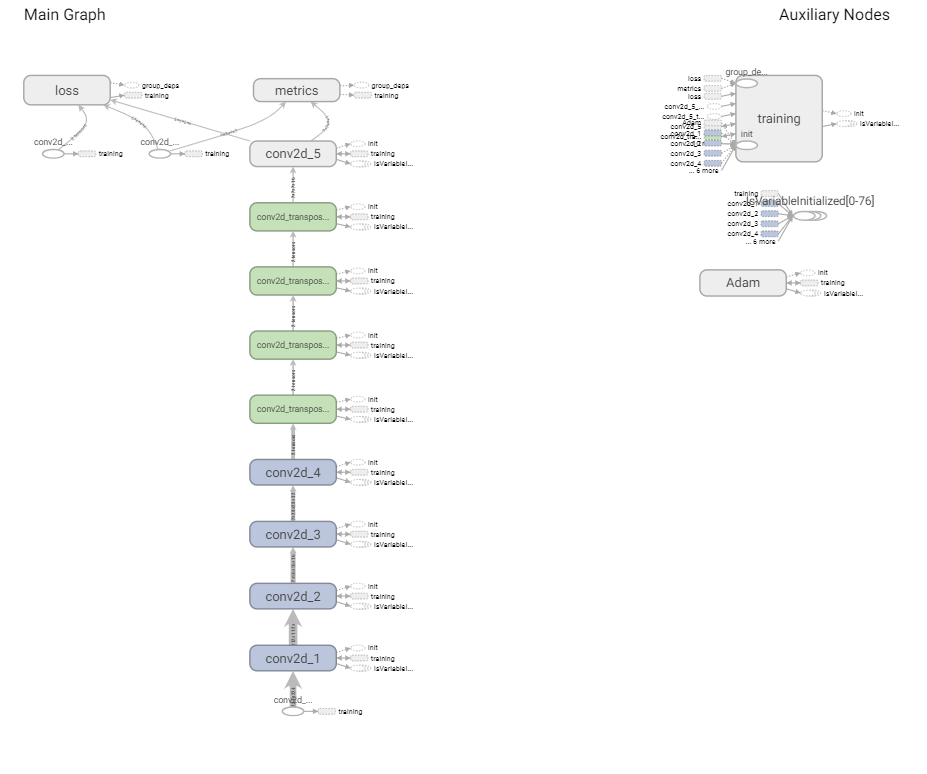
\includegraphics[width=0.8\textwidth]{bilder/tensorboard_graph.PNG}
    \caption{The model graph visualized in Tensorboard}
    \label{fig:graph}
\end{figure}
The other section in Tensorboard called \textit{"GRAPHS"} shows the model graph. Being able to see the layers, optimizer function and connections, helps the user see the whole model in a better perspective. There is possible to rename each layer in the model according to the user's own request. 
\section{Convolutional neural networks}
\subsection{Filters}
\subsection{Relu}
\subsection{Layers}
\subsection{Activation layers}
\subsection{Loss}
\subsection{Optimizers}
\subsubsection{Regularization}
\section{Active learning}
\subsection{Predictions}
\subsection{Threshold}
\subsection{Morphological operations}
The most common binary image operations are called \textit{morphological operations}, since
they change the shape of the underlying binary objects \cite{Ritter}. This is done by convolving a binary \textit{structuring element} on the binary image, where the structuring element can be any chosen shape. These operations are typically used to clean up binary images, and two of the standard binary morphological operations used in our project are: 
\begin{itemize}
    \item \textbf{Erosion}
    \item \textbf{Dilation}
\end{itemize}

Where \textit{erosion} thins the object and \textit{dilation} thickens the object. As one may notice, there is some noise in the thresholded image in figure \todo{fig:seg}, which is a consequence of thresholding an image by color. Using these operations in this specific order (erosion + dilation) results in \textit{opening}. This operation tends to close large regions, smooth boundaries, while removing the noise (white dots) as shown in the figure \todo{fig:morph}. The program erodes twice to remove white dots, then do five dilations to fill the contours, making them more visible in the segmented image. The structuring element used is a 3x3 rectangular kernel.

\subsection{Connected component analysis}
\subsection{Annotating the data set}
When the training set needs to labeled, there is quite a few options to choose a suitable program. Most of them is online driven, meaning the data set needs to be uploaded to a website, and the annotation can further be done from there. A program which offer offline annotation is called \textit{"labelme"}\cite{website:labelme}. 
\subsection{Choosing the right images for further training}
\subsection{Train again}
\section{Related works}
\newpage
\chapter{Method}
\section{Annotation the training set}


\chapter{Results}                     

\chapter{Discussion}



\backmatter{}
\printbibliography
\end{document}
